\section{实验结果及其分析}

\subsection{数据集来源}
本文采用自建数据库,使用java web页面进行数据录入,如图6-1所示:

\begin{figure}[thbp!]
	\centering
	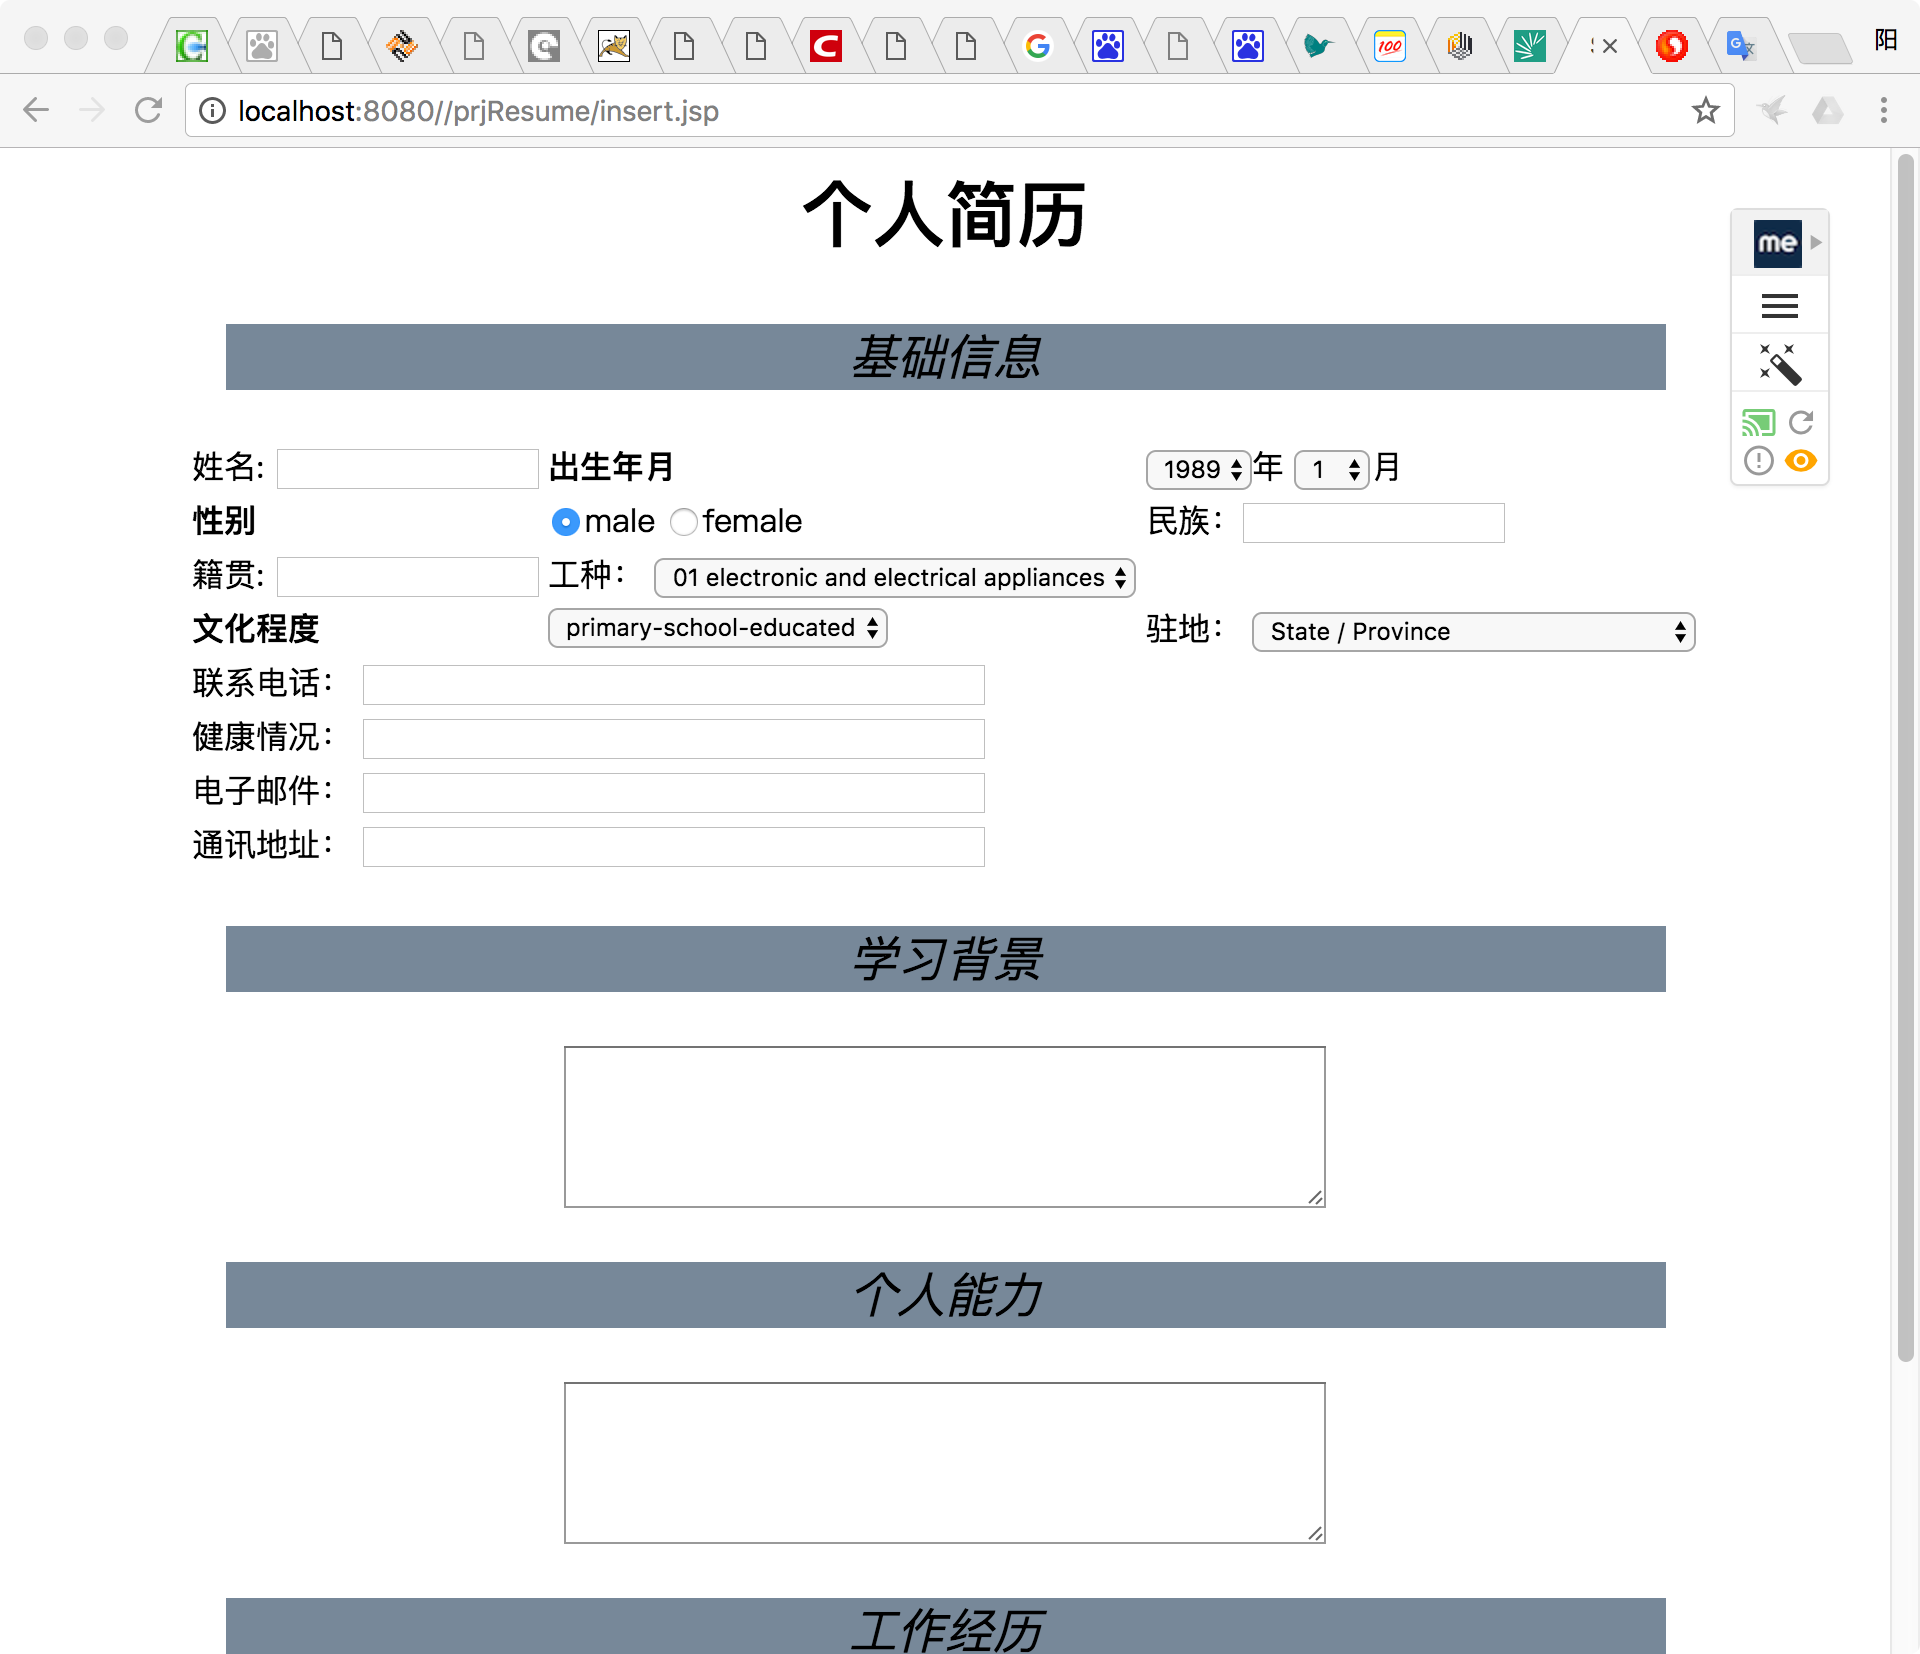
\includegraphics[width=0.4\linewidth]{figure/6-1}
	\caption{数据录入}
	\label{fig:6-1}
\end{figure}

提取mysql数据库中供给的数据集。

依据inf表,选用对应数据作为实验数据集,然后根据数据反映情况进行数据决策树生成及最终完成预测。

\subsection{度量标准}
本文的目的是针对海量数据的异常项检测及分类方法研究完成最终的预测行为,从而对未来的数据处理进行有针对性的指导。质量的度量标准主要包括统计精度度量方法和决策支持精度度量方法两类。统计精度度量方法中的平均绝对偏差MAE(mean absolute error)易于理解,可以直观地对推荐质量进行度量,是最常用的一种推荐质量度量方法,本文采用平均绝对偏差MAE作为度量标准.平均绝对偏差MAE通过计算预测的用户评分与实际的用户评分之间的偏差度量预测的准确性,MAE越小,推荐质量越高。

设预测的用户评分集合表示为${p_1,p_2,p_3,...,p_n}$,对应的实际用户评分集合为${q_1,q_2,q_3,...,q_n}$,则平均绝对偏差MAE定义为:

\begin{equation}
MAE=\frac{\sum_{i=1}^n |p_i-q_i|}{n}
\end{equation}

\subsection{用户分类}
对于用户信息,根据用户属性之间关联性,将用户通过数据规则自动分类。

\subsubsection{用户信息统计}
此次,涉及数据信息属性有三个,分别是major,residence,status依据预处理之后的信息数据,得知此次总共调查了40个数据集的信息。

\subsection{数据预测}

\subsubsection{数据预测准备}
 经过之前的多级数据处理后我们可以都到关于驻地跟文化程度两个关于驻地,专业,文化程度的决策树,以此为前提,我们使用RapidMiner的相关算子进行对应的数据预测。

\subsubsection{数据预测操作}
使用之前处理过的数据,并在其后添加算子Apply Model如图6-2:

\begin{figure}[thbp!]
	\centering
	\includegraphics[width=0.4\linewidth]{figure/6-2}
	\caption{添加算子 Apply Model}
	\label{fig:6-2}
\end{figure}

运行Process,可以得到如下的预测图:

\begin{figure}[thbp!]
	\centering
	\includegraphics[width=0.4\linewidth]{figure/6-3}
	\caption{预测图}
	\label{fig:6-3}
\end{figure}

图6-3反应了对不同文化程度对应不同驻地的预测,例如:小学文化程度对应驻地为省级的概率为20%

\begin{figure}[thbp!]
	\centering
	\includegraphics[width=0.4\linewidth]{figure/6-4}
	\caption{预测图2}
	\label{fig:6-4}
\end{figure}

图6-4以条形图的方式反应出不同的文化程度对应不同工种的预测比例,其中不同的工种代表不同的颜色,对应在不同文化程度的条形图中分布比例。

\begin{figure}[thbp!]
	\centering
	\includegraphics[width=0.4\linewidth]{figure/6-5}
	\caption{预测图3}
	\label{fig:6-5}
\end{figure}

图6-5反应出不同工种对应不同驻地的预测,例如:省级驻地对应07 高科技类工种跟02 管理类工种的概率均很高

\begin{figure}[thbp!]
	\centering
	\includegraphics[width=0.4\linewidth]{figure/6-6}
	\caption{预测图4}
	\label{fig:6-6}
\end{figure}

图6-6反应出不同文化程度对应不同工种的预测,例如:本科文化程度对应从事02 管理类工种的概率就很高

\subsection{实验结果分析}
依照上述数据预测结果,我们可以得到不同文化程度对应不同驻地的预测值(confidence),以及不同工种对应不同驻地的预测值,不同文化程度对应不同专业的预测值。即通过对样本数据的异常项检测及分类方法研究,实现了数据属性之间的相似性度量研究,并通过决策树算法产生基于样本数据的预测算法,实现数据的利用最大化。